\section{Optimizations}\label{sec:opt}
\name performs many of the standard compiler optimizations,
such as Dead Code Elimination and Constant Propagation.
Some of them, however, plays a much more important rule for reconfigurable accelerator because they
have direct impact on the resource usage.
Other optimizations can be counter-intuitive, as they introduce redundant computation that
reduces resource without necessarily impacting performance.
In this discussion, we focus our primary objective on performance.
Resource is an indirect objective as resource reduction enable larger parallelization factors,
, which in turn improves performance.

\subparagraph{Memory strength reduction (msr).} Like traditional strength reduction on arithmetics, \name{} replaces expensive on-chip memories with cheaper memories whenever possible.
%We map register accumulation in the program with single-cycle initiation interval to pipeline registers.
For example, \name{} replaces a scratchpad with constant address in all accesses to a un-indexable memory, such as a FIFO.
This commonly happens when producer and consumer loops of the memory are fully unrolled.

\subparagraph{Route-Through Elimination (rtelm).} For patterns where the content of a non-indexable memory  (M1) is read and written to another memory (M2), \name{} eliminates the intermediate access if the read of M1 and the write of M2 operates in lock-step.

\begin{figure*}
\centering
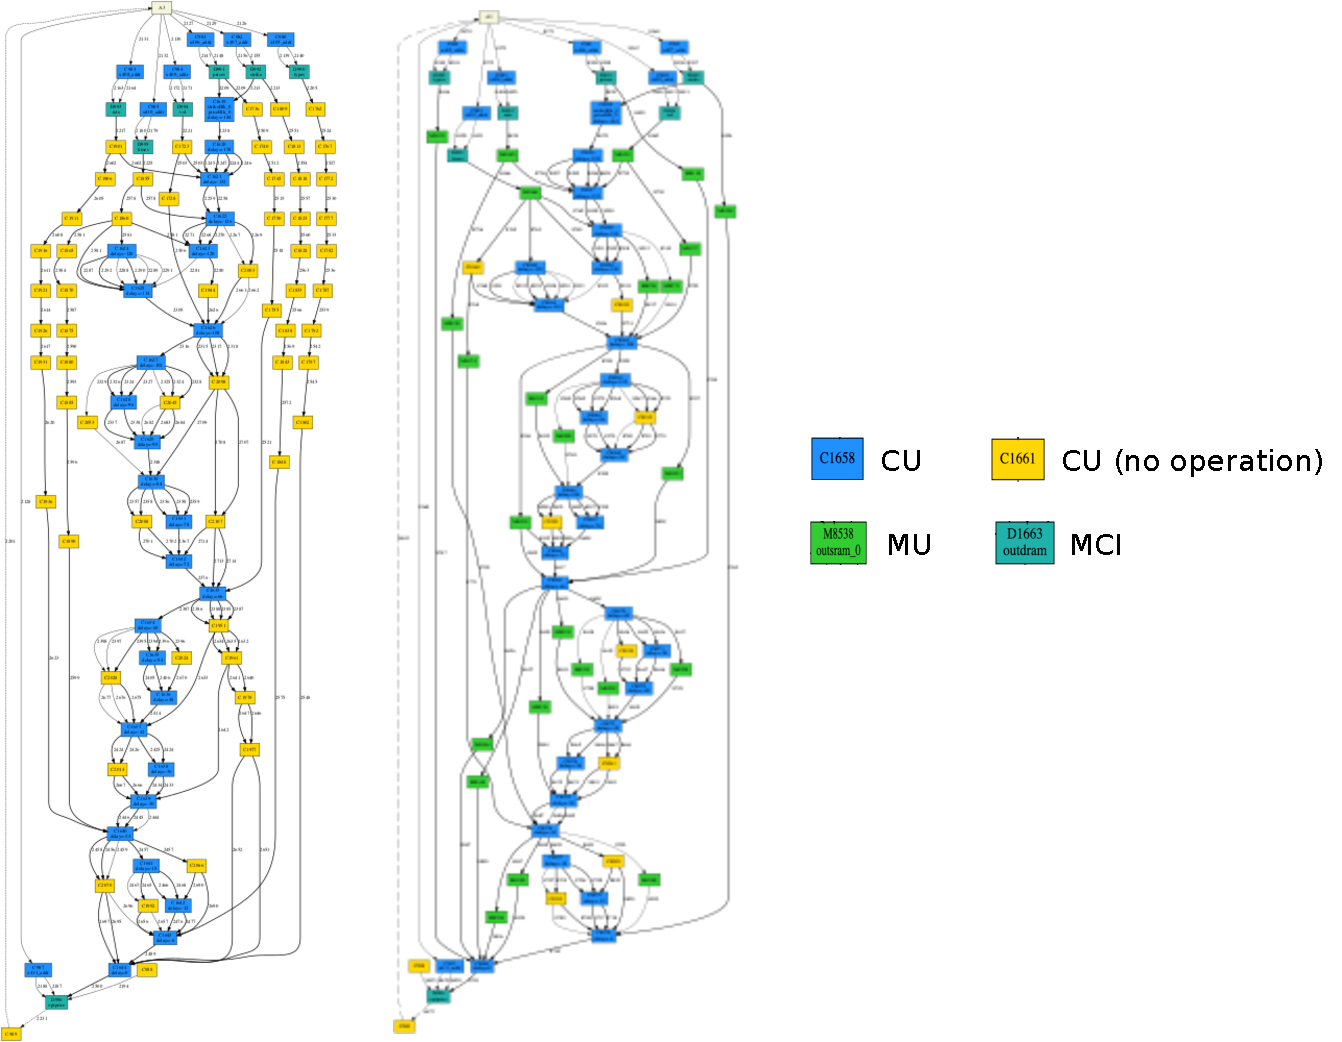
\includegraphics[width=0.7\textwidth]{figs/retiming.pdf}
\caption[Retiming]{
  Left: retiming with input buffer only. Right: retiming with either input buffer or scratchpad.
}
\label{fig:mlp}
\end{figure*}
\subparagraph{Retiming with scratchpad (retime-mem).} By default, \name{} uses PB input buffers for retiming purpose. 
This option enables \name{} to use scratchpad memory for retiming that requires large buffer depth.

\subparagraph{Crossbar datapath elimination (xbar-elm).}
Although, crossbars between accessors and memory partitions (\Cref{sec:memsplit}) are very expensive in the general case, the BI sometimes can be statically resolvable with certain combinations of parallelization on memory accesses. 
When BI is a constant, \name{} can use this information to intelligently assign virtual banks to partitions that reduce the crossbar data path to a partial or a point-to-point connection.

\subparagraph{Read request duplication (dupra).} During memory partitioning (\Cref{sec:memsplit}), instead of forwarding BI from the requester to receiver, \name{} can also duplicate the BI with local state on receiver side, which
eliminates the unbalanced data path at the cost of extra computation.

\begin{figure*}
\centering
\begin{subfigure}[b]{0.6\textwidth}
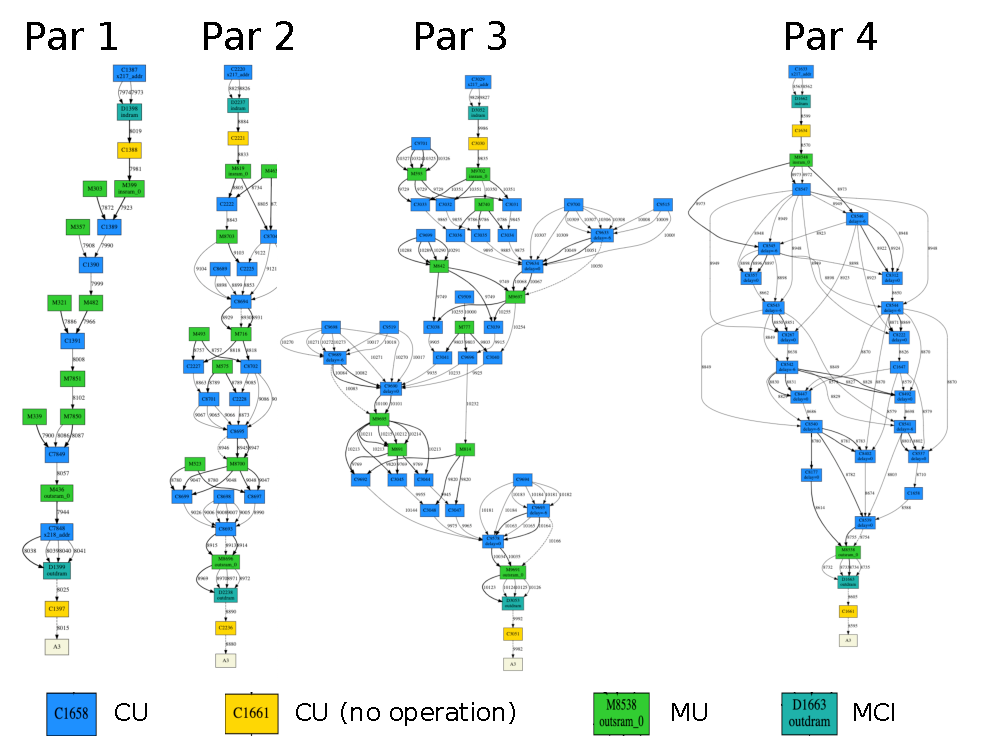
\includegraphics[width=1\textwidth]{figs/mlpunroll.pdf}
\caption{VUDFGs with different parallelization factors}
\end{subfigure}
\hfill
\begin{subfigure}[b]{0.39\textwidth}
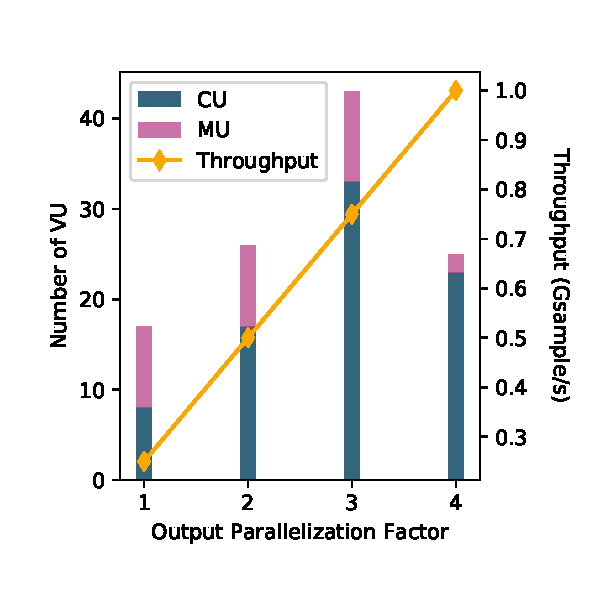
\includegraphics[width=1\textwidth]{figs/mlp.pdf}
\caption{Throughput and resource as a function of parallelization factor}
\end{subfigure}
\caption[MLP case study]{
  MLP case study
}
\label{fig:mlp}
\end{figure*}

\subparagraph{Global Merging (merge).}
After all VBs satisfy the hardware constraint, we perform a global optimization to compact small VBs into  larger VBs. 
Merging has very similar problem statement as compute partitioning (\Cref{sec:compsplit}) except with more constraints.
The traversal-based algorithm requires a reference cost for PB to check if the merged VB still satisfy the hardware constraint.
At each step of merging, we take the union of the domains of VBs within the current partition, and intersect with the domain of the merging VB.
The caveat is that even with a non-empty intersection, the bipartite graph might not have a possible assignment, as merged VB might fit in a larger PB with insufficient quantity.
Therefore, we perform a heuristic checking on feasibility of the bipartite assignment at each step of merging.
The solver-based solution combines partition assignment with PB type assignment as a joint problem. 
The output of merging gives both partition assignment as well as a PB type assignment, which eliminates the risk of un-mappable bipartite graph due to merging in the traversal-based solution.

\subparagraph{Memory Localization}
We perform another specialization on non-indexable memories (registers or FIFOs), whose all accesses have no explicit read enables.
Instead of treating them as shared memories, \name{} duplicates and maps them to local input buffers in all receivers, no longer requiring tokens.
The sender actor pushes to the network when the token is supposed to be sent, and the receiver dequeues one element from the input buffer when the token is supposed to be consumed.
This dramatically reduces the synchronization complexity of non-indexable memory in the common case.

\subparagraph{Reverse Loop Invariant Hoisting}
A common loop optimizations is to move loop invariant expressions outside of the loop body to reduce
computation. This optimizations, however, might introduce more basic blocks in the program.
For Plasticine, number of basic blocks have a strong correlation with number of contexts and
physical units. \Cref{fig:reversehoisting} shows an example where moving instructions into the loop
body reduces number compute units. Because instructions within basic blocks and basic blocks
themselves are pipelined, doing so does not have performance impact on the application.
Currently, we rely on the user to perform manually perform this optimization.

\begin{figure*}
\centering
\hfill
\begin{subfigure}[b]{0.4\textwidth}
\inputminted{python}{code/hoisting.py}
\caption{Input program}
\end{subfigure}
\hfill
\begin{subfigure}[b]{0.4\textwidth}
\inputminted{python}{code/reversehoisting.py}
\caption{Reverse Loop Invariant Hoisting}
\end{subfigure}
\hfill
\caption[Reverse Loop Invariant Hoisting]{
  The original program requires at least two contexts to execute Block 1 and Block 2.
  By moving the invariant instruction \texttt{c = a + b} into the loop body, (b) only needs a single
  context instead. Because instructions within \texttt{Block 2} are pipelined across loop
  iterations, adding instructions in the loop body introduce minimum performance impact.
  This transformation is beneficial until \texttt{Block 2} exceeds six operations, at which point
  both version consume the same amount of resources.
}
\label{fig:reversehoisting}
\end{figure*}

\begin{figure*}
\centering
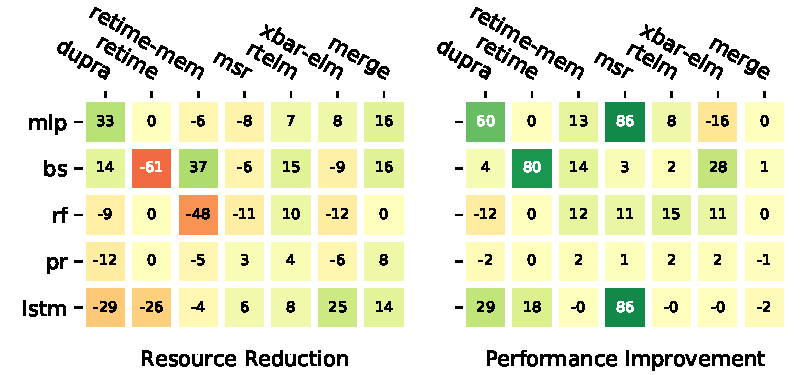
\includegraphics[width=0.7\textwidth]{figs/heat.pdf}
\caption[Optimization Effectiveness]{
  Optimization Effectiveness. Percentage resource reduction or performance improvement from each
  optimization. The heat map shows the maximum differences when turning on/off the optimization, 
  while keeping other optimizations the same.
  For a single application, the improvement is taking the geometric mean across different application parameters.
}
\label{fig:reversehoisting}
\end{figure*}
%\subparagraph{Dead Code Elimination (DCE)} 
%We perform aggressive DCE on the VBDFG and only keeps computation that gets materialized to accelerator I/O and DRAM.
%\subparagraph{Constant Propagation}
%Aside from regular constant propagation on arithmetics, we also eliminates crossbar datapath when bank ID 
%can be statically resolved described later in \Cref{sec:memsplit}.
%During loop unrolling, address of indexable memory sometimes can be resolved to static constant.
%For a read-only RAM with constant address, we lookup their content at compile time and embed its content into registers.
%For \emph{route-through} pattern, where content of a non-indexable memory M1 is read and written to another memory M2,
%we can eliminate the intermediate write and forward the data directly to the final memory if the compiler
%can prove the read M1 and write of M2 operates in lock-step.
%We also perform constant propagation on control signals with loop-range analysis. 
%Eliminates the control signals can expose more lock-step accesses and \emph{route-through} opportunities.
%\subparagraph{Strength Reduction}
%In addition to traditional strength reduction on arithmetics, we also replace expensive memories
%with cheaper memory whenever possible.
%We map register accumulation in the program with single-cycle initiation interval to pipeline registers.
%Banked-SRAM with constant bank IDs and offsets in all accessors can also be replaced with FIFOs,
%which is happens when producer and consumer loops are fully unrolled.

%Accesses statically banked in the input graph can operates concurrently 
%without bank conflicts, as explained in \Cref{sec:background}.
%These accesses are usually from a unrolled loops. For banked accesses from the same pre-unrolled access, 
%\name first merge all requests before sending to the memory (details in \Cref{sec:memsplit}). 
%Because these accesses are from loop unrolling, they have the same program order and same dependency with other accesses.
%So the synchronization can be performed on the merged access, which prevents the amount of synchronization
%to increase with parallelism on a banked memory, as shown in \Cref{fig:mergetoken}

%\subsubsection{Blackbox IP Pruning} \label{sec:bbsplit}
%\yz{Cut this if out of the space}
%This step illustrates an example of integrating a customized partitioner for composable IP available on
%the architecture.
%The cost metrics and partition rule is specific to each IP.
%The example IP is a merge buffer, which can merge two sorted vector streams into a single stream with
%one vector per cycle throughput.
%The merge buffer pruner uses a tree of 2-way merge buffers across PBs to compose a multi-way merge buffer declared in the program.


